\documentclass[11pt]{article}

\usepackage[margin=1in]{geometry}
\usepackage{amsmath,amssymb}
\usepackage{booktabs}
\usepackage{graphicx}
\usepackage{microtype}
\usepackage{parskip}
\usepackage{xcolor}
\usepackage{hyperref}
\usepackage{fancyhdr}
\usepackage{caption}

\definecolor{ava}{HTML}{3569A8}
\definecolor{avb}{HTML}{D06B32}
\definecolor{accent}{HTML}{9E2449}

\hypersetup{
  colorlinks=true,
  linkcolor=accent,
  urlcolor=ava,
  pdftitle={Why the AVA and AVB Drive Onsets Are SNICs},
  pdfauthor={Distribution of Oscillators Project}
}

\pagestyle{fancy}
\fancyhf{}
\fancyhead[L]{\small Distribution of Oscillators}
\fancyhead[R]{\small AVA/AVB drive bifurcations}
\fancyfoot[C]{\thepage}
\setlength{\headheight}{14pt}

\captionsetup{font=small,labelfont=bf}

\title{Why the AVA and AVB Drive Onsets Are SNICs\\
\large Equilibrium stability and infinite-period scaling in the 17-cell segment}
\author{Distribution of Oscillators Project}
\date{August 18, 2026}

\begin{document}

\maketitle

\begin{abstract}
We classify the onset of rhythmic activity in the 17-cell \textit{C.~elegans}
segment as either AVA or AVB command current is increased from zero. In both
branches, the resting equilibrium terminates when a real eigenvalue reaches
zero, a finite-amplitude periodic orbit exists immediately above the same
current, and its period follows the inverse-square-root divergence expected at
a saddle-node bottleneck. The combined evidence identifies both onsets as
saddle-node-on-invariant-circle (SNIC) bifurcations rather than Hopf or
saddle-homoclinic transitions.
\end{abstract}

\section{Question and model}

The question is not merely where oscillation begins, but what local and global
dynamics create it. We therefore combine equilibrium continuation, Jacobian
eigenvalues, direct periodic-orbit measurements, and near-onset scaling.

The calculation uses the reduced 34-state $(V,w)$ representation of the full
17-cell segment. Synaptic fatigue is excluded because it currently evolves
without multiplying the synaptic signal and therefore cannot affect the
voltage-recovery bifurcation. AVA and AVB are studied separately: one command
current is varied while the other is held at zero.

The controlled parameter set is
\begin{align*}
G_{\mathrm{syne}} &= 0.07\ \mathrm{nS}, &
G_{\mathrm{syni}} &= 0.05\ \mathrm{nS}, &
G_{\mathrm{gap}} &= 0.03\ \mathrm{nS}, \\
k_{\mathrm{syn}} &= 0.25\ \mathrm{mV}^{-1}, &
V_{\mathrm{th}} &= -52\ \mathrm{mV}, &
\beta &= 1.03, \qquad \tau_w=400\ \mathrm{ms}.
\end{align*}

The value $\tau_w=400$ ms is the canonical baseline selected on
2026-08-25 from a controlled AVA/AVB dorsoventral-phase sensitivity sweep.
The original 2026-08-18 calculation used 200 ms; recomputation at 400 ms
preserves the equilibrium fold locations and SNIC classification while
changing the realized cycle timescale and muscle output.

\section{Numerical result}

The resting equilibrium terminates at
\begin{equation}
\boxed{I_{\mathrm{SN}}^{\mathrm{AVA}}=1.68143\ \mathrm{pA}},
\qquad
\boxed{I_{\mathrm{SN}}^{\mathrm{AVB}}=1.59643\ \mathrm{pA}}.
\end{equation}

Table~\ref{tab:evidence} summarizes the independent numerical signatures.

\begin{table}[ht]
\centering
\caption{Evidence used to classify the lower command-drive bifurcations.}
\label{tab:evidence}
\renewcommand{\arraystretch}{1.18}
\begin{tabular}{@{}lcc@{}}
\toprule
Diagnostic & \textcolor{ava}{AVA} & \textcolor{avb}{AVB} \\
\midrule
Fitted onset current $I_{\mathrm{SN}}$ (pA) & 1.68143 & 1.59643 \\
Fold fit $R^2$: $\lambda^2\propto I_{\mathrm{SN}}-I$ & 0.99997 & $>0.999999$ \\
Functional amplitude observable & $\Delta_{DV}$ & $\Delta_{DV}$ \\
Near-onset DV amplitude (mV) & $\approx47.6$ & $\approx47.7$ \\
Period at $\Delta I=0.025$ pA (s) & 3.37 & 3.46 \\
Period at $\Delta I=0.0001$ pA (s) & 18.08 & 18.66 \\
Fit $R^2$: $T=A/\sqrt{\Delta I}+B$ & 0.99950 & 0.98774 \\
\bottomrule
\end{tabular}
\end{table}

\section{Evidence 1: the equilibrium has a saddle-node}

Figure~\ref{fig:equilibrium} follows the stable resting state as command drive
increases. The branch terminates at a fold. In the lower panels, the critical
eigenvalue is purely real and approaches zero. The near-fold relation
\begin{equation}
\lambda^2 \propto I_{\mathrm{SN}}-I
\end{equation}
has essentially unit coefficient of determination for both commands, as
expected for a generic saddle-node. This establishes the ``SN'' part of SNIC.

\begin{figure}[p]
\centering
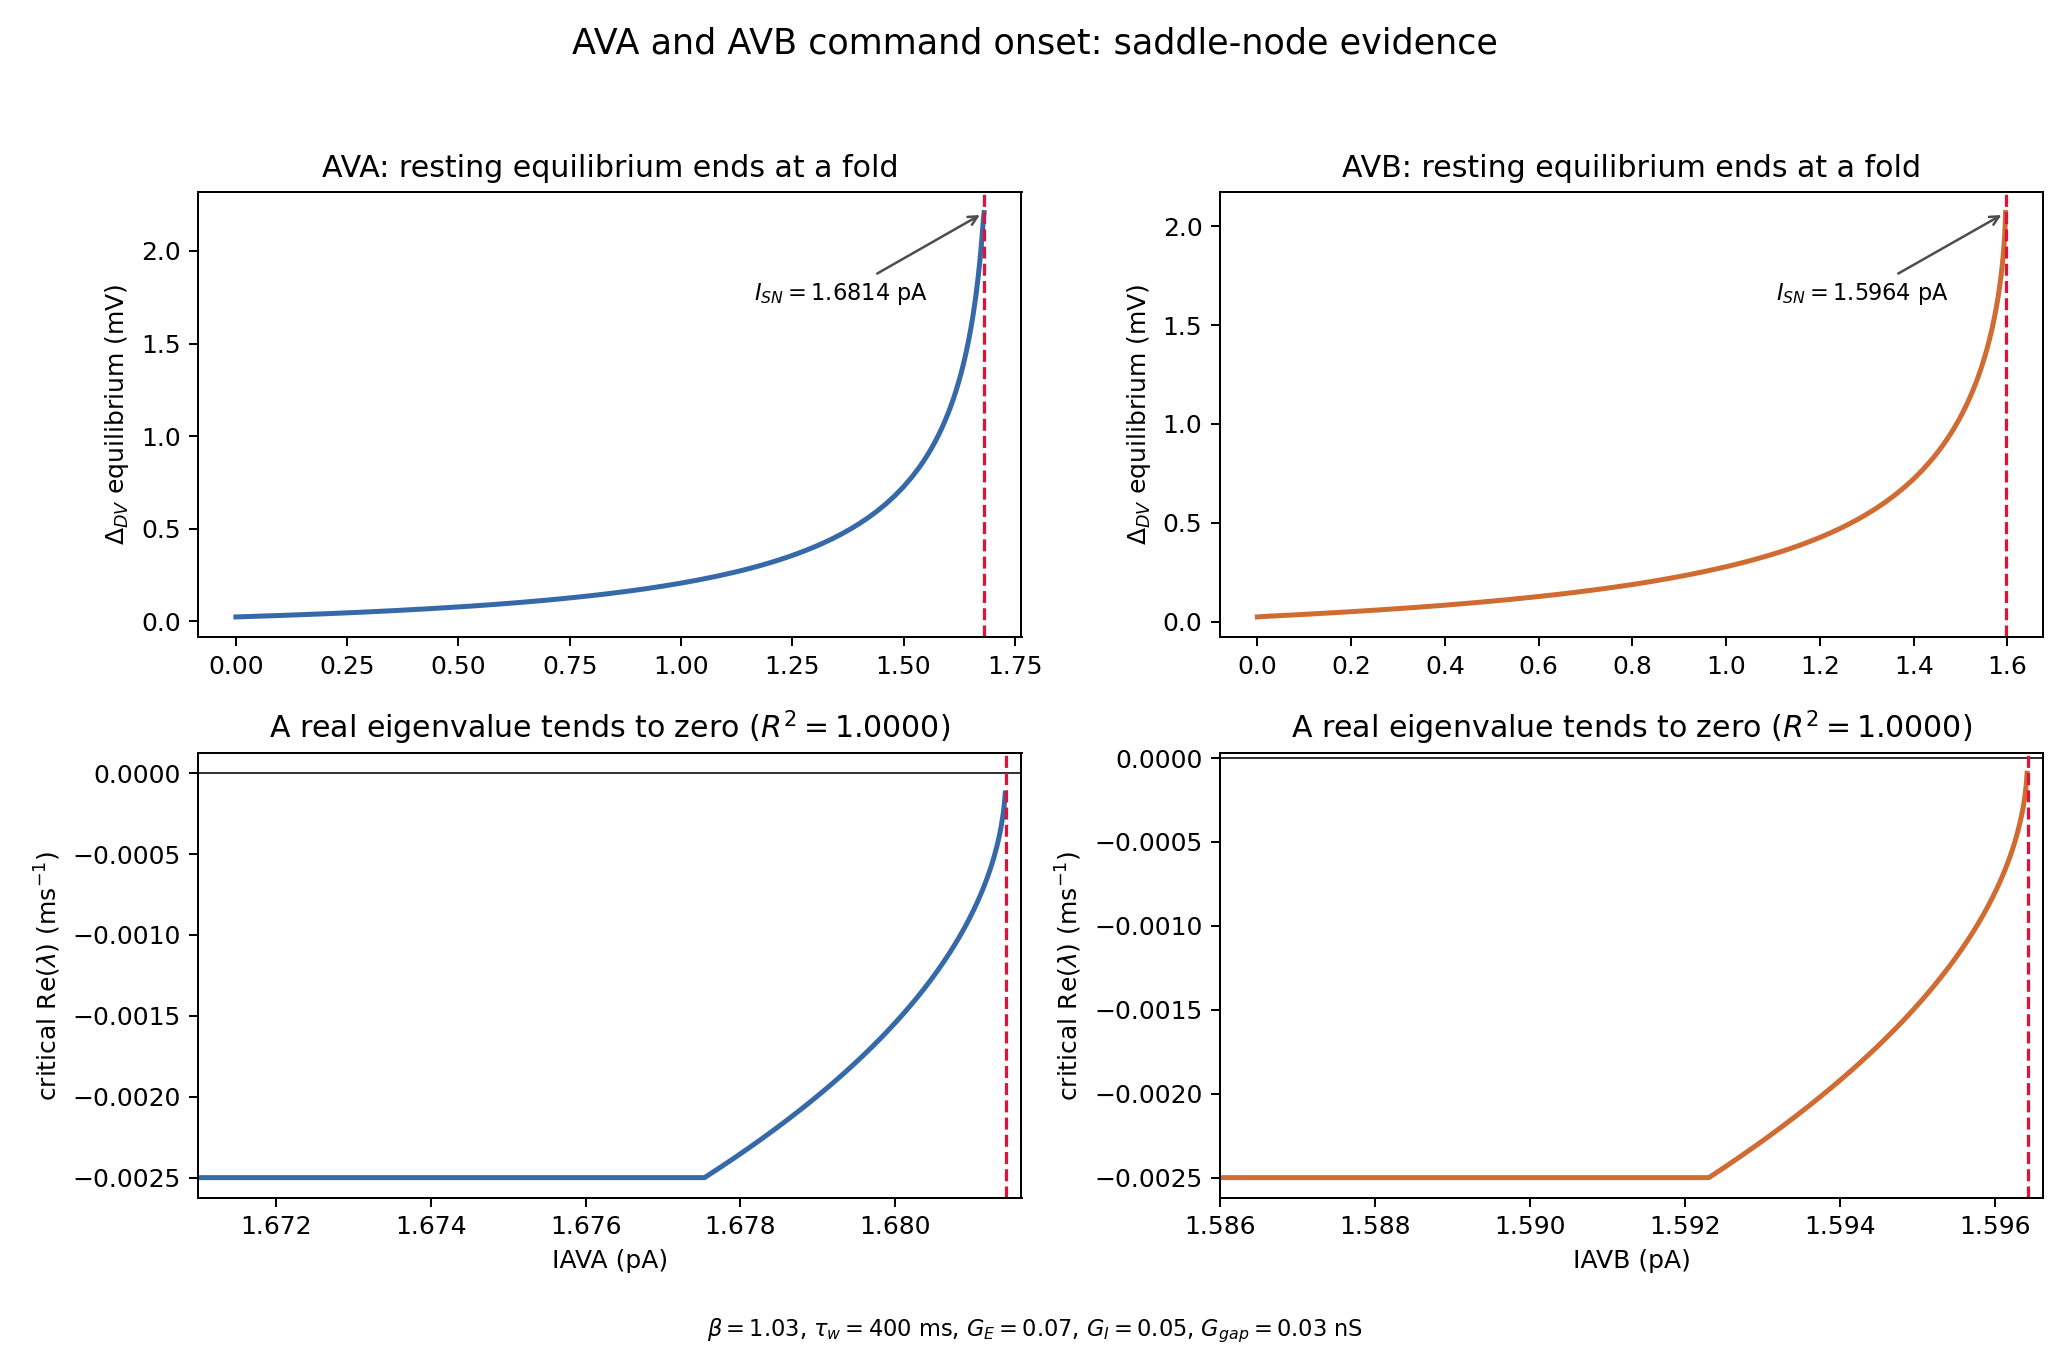
\includegraphics[width=\textwidth]{../../media/bifurcation_drive_snic_equilibrium.png}
\caption{Equilibrium and eigenvalue evidence. The stable resting branch ends at
the marked command current. A real eigenvalue, rather than a complex conjugate
pair, tends to zero at each fold. The lower panels magnify the last 0.01 pA
below onset.}
\label{fig:equilibrium}
\end{figure}

\clearpage
\section{Evidence 2: a finite-amplitude cycle has infinite period}

Stable periodic activity exists immediately above each equilibrium fold. Its
functional dorsoventral excursion remains approximately 48 mV as
$\Delta I=I-I_{\mathrm{SN}}$
approaches zero, so the orbit does not collapse onto a small-amplitude
oscillation. Instead, the period grows from roughly 3.4 s to 18--19 s over the
sampled interval.

The orbit therefore retains its global geometry while spending progressively
more time near the location of the vanished equilibria. The fitted law
\begin{equation}
T(\Delta I)=\frac{A}{\sqrt{\Delta I}}+B
\end{equation}
describes the command branches with $R^2=0.99950$ (AVA) and $0.98774$ (AVB); see
Figure~\ref{fig:cycles}. The additive constant $B$ is the regular traversal
time around the portion of the orbit away from the saddle-node bottleneck.

\begin{figure}[p]
\centering
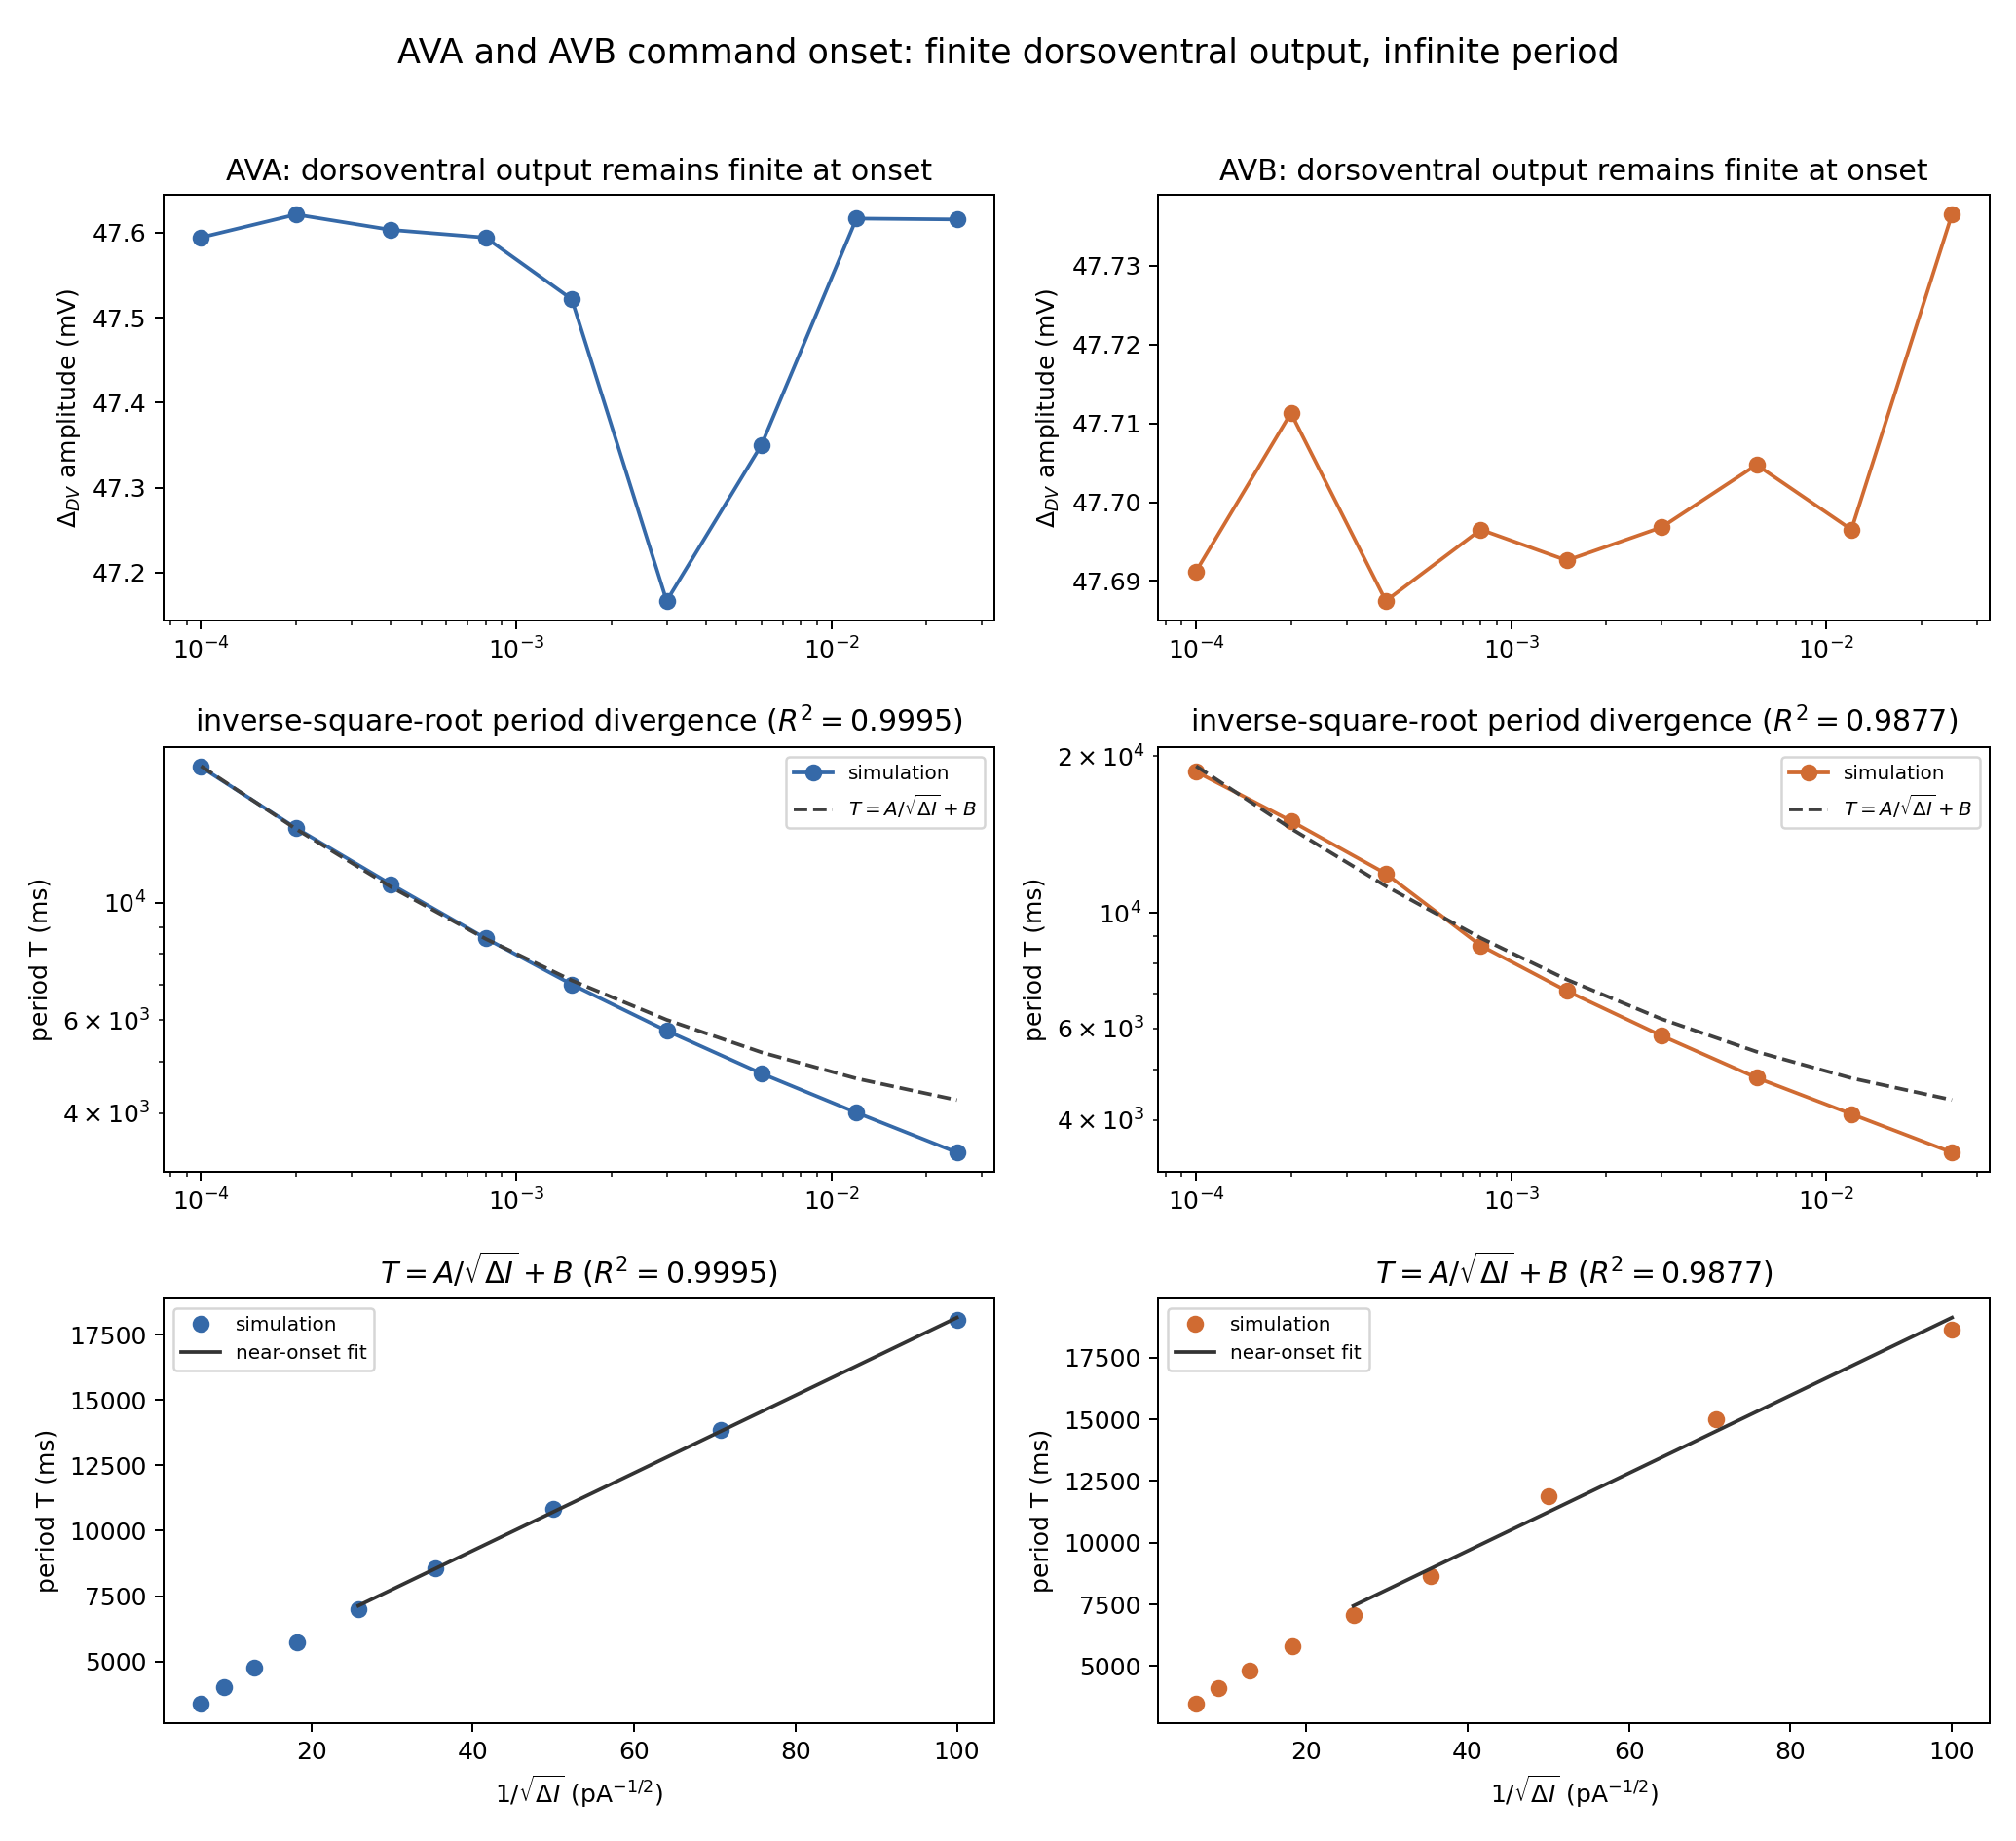
\includegraphics[width=0.97\textwidth]{../../media/bifurcation_drive_snic_cycles.png}
\caption{Periodic-orbit evidence. Top: cycle amplitude remains finite near
onset. Middle: the period diverges as the drive approaches the fold. Bottom:
period is linear in $1/\sqrt{\Delta I}$ over the five closest samples.}
\label{fig:cycles}
\end{figure}

\clearpage
\section{Why inverse-square-root scaling identifies a SNIC}

Near a generic saddle-node, the flow along its center direction has the normal
form
\begin{equation}
\dot{x}=\mu+a x^2,
\qquad
\mu=I-I_{\mathrm{SN}}.
\end{equation}
For $\mu>0$, the equilibria have disappeared but trajectories still pass
slowly through their former location. The bottleneck traversal time is
\begin{equation}
T_{\mathrm{bottleneck}}
\sim
\int_{-\infty}^{\infty}\frac{dx}{\mu+a x^2}
=\frac{\pi}{\sqrt{a\mu}}.
\end{equation}
Adding the finite time required to traverse the rest of the orbit gives
$T=A/\sqrt{\mu}+B$. Thus
\begin{equation}
T\longrightarrow\infty,
\qquad
f=\frac{1}{T}\sim\sqrt{I-I_{\mathrm{SN}}}\longrightarrow0,
\end{equation}
even though the voltage amplitude remains large.

This is precisely what the simulations show. The periodic trajectory passes
through the saddle-node bottleneck and closes globally, so the saddle-node lies
on the invariant circle traced by the limiting orbit.

\section{Why the main alternatives are rejected}

\begin{description}
\item[Hopf bifurcation.]
A Hopf transition requires a complex conjugate eigenvalue pair to cross the
imaginary axis. Here the critical eigenvalue is real. A Hopf also has a finite
linear onset frequency, whereas the measured frequency tends to zero.

\item[Saddle-homoclinic bifurcation.]
A homoclinic orbit also has an infinite period, but its leading divergence is
logarithmic, $T\sim-C\log(\Delta I)$, rather than inverse-square-root. It also
does not require the periodic orbit to terminate at the observed equilibrium
fold. The measured $T=A/\sqrt{\Delta I}+B$ scaling and fold coincidence support
a SNIC instead.
\end{description}

The classification is therefore based on four mutually reinforcing facts: a
saddle-node in the equilibrium branch, a real critical eigenvalue, a
finite-amplitude cycle immediately above the same current, and the SNIC
infinite-period scaling law.

\section{Reproduction and outputs}

From the repository root, run
\begin{verbatim}
conda activate simple-worm-scripts
python experiments/drive_snic.py
\end{verbatim}

The script generates the two figures used here and
\path{media/bifurcation_drive_snic_results.json}. The JSON record contains every
sampled drive, period, frequency, DV amplitude, period method, period CV,
fitted fold, and goodness-of-fit statistic.

\end{document}
